% =============================================================================
%  SIA: Surface-Isomorphic Abstention -- Learning to Say "I Don't Know"
%
%  This is the focused paper: criterion + method + controlled experiment.
%  It was split out of the 18-page version (SIA_paper.tex), which additionally
%  reported a real-knowledge-boundary construction, its failure on this same
%  criterion, an item-level cost analysis, a taxonomy of measurement failures
%  and a GRPO boundary. Those belong to a companion and are not repeated here;
%  section 6 says where they went and why.
%
%  All numbers are unchanged from the experiment record. Source is pure ASCII
%  and builds with pdfLaTeX or XeLaTeX on a stock TeX Live.
%
%  Compile: pdflatex SIA_abstention.tex   (twice)
% =============================================================================
\documentclass[11pt,a4paper]{article}

\usepackage[T1]{fontenc}
\usepackage[utf8]{inputenc}
\usepackage[margin=2.4cm]{geometry}
\usepackage{amsmath,amssymb}
\usepackage{booktabs}
\usepackage{graphicx}
\usepackage{adjustbox}
\usepackage{array}
\usepackage{enumitem}
\usepackage{url}
\urlstyle{tt}
\usepackage{caption}
\usepackage{multirow}
\usepackage{xcolor}
\usepackage[colorlinks=true,linkcolor=blue!55!black,citecolor=blue!55!black,
            urlcolor=blue!55!black]{hyperref}

\captionsetup{font=small,labelfont=bf}
\setlength{\tabcolsep}{4.5pt}
\setlength{\emergencystretch}{2em}
\newcommand{\good}[1]{\textcolor{green!45!black}{\textbf{#1}}}
\newcommand{\bad}[1]{\textcolor{red!70!black}{\textbf{#1}}}
\newcommand{\surfcv}{$\mathrm{surf}_\mathrm{CV}$}

\title{\bfseries SIA: Surface-Isomorphic Abstention\\[6pt]
\large Learning to Say ``I Don't Know''}

\author{Sen Song\\ \small Independent Researcher, Guangzhou, China}
\date{}

\begin{document}
\maketitle

\begin{abstract}
\noindent
Large language models hallucinate most readily where they have no evidence: no
ground truth exists to shape a reward and no retrievable evidence exists in
context. We treat abstention there as a class to be learned rather than a
question of correctness, and we ask what makes its training data work.

We give a falsifiable criterion. \emph{Counter-example completeness} is stated
relative to the surface features that training and evaluation share: no rule
expressible in those features may fit the training set better than chance. It
comes with a test needing only the training set and no ground truth, the
cross-validated accuracy \surfcv{} of a surface-only discriminator.

We present \textbf{SIA} (\emph{Surface-Isomorphic Abstention}), a four-step
recipe that teaches answers and abstentions with ordinary supervised
fine-tuning: $94$\,s per arm, no reward model, no RL loop. On a controlled
construction that passes the test (\surfcv{} lands on the majority baseline, a
gap of $-0.000$), SIA drives the fabrication rate on unseen entities and unseen
phrasings from $0.933$ to \textbf{0.000} and abstention from $0.000$ to
\textbf{1.000}, with verifiable capability unchanged. The criterion has teeth:
three conditions originally read off practice---that the two slices share
surface structure, that abstention and answer examples share templates, and
that there be at least three unknown entities---are its three axes, and
breaking any one of them collapses the effect to exactly $0.000$, while a
compute-matched control rules out extra training and a positive control on
abstention-only training shows that abstention transfer is not the hard part.

The construction also shows something on its own. When one slice has no gold
answers, aggregate accuracy is not merely insensitive but anti-correlated with
safety, because a confident error and a safe abstention are scored identically.
Stratified reporting is not a stylistic choice here.
\end{abstract}

\noindent\textbf{Keywords:} hallucination mitigation; abstention learning;
knowledge boundary; supervised fine-tuning; shortcut learning

\section{Introduction}
\label{sec:intro}

\subsection{The problem}

Hallucination takes several forms. We address one: the model has no stable
internal information about a given (entity, attribute) pair and produces a
specific answer anyway. We call such items the \emph{evidence-free slice}.
Three neighbours are out of scope: facts taught but misremembered; facts for
which evidence exists but is overridden by context; and errors the model holds
self-consistently. Those belong to retrieval and to RL.

The evidence-free slice is hard for two structural reasons. First, there is no
reliable ground truth: what the correct answer is for a long-tail item is often
unknown even to annotators, so any reward that depends on grading correctness,
verifiable rewards included, is undefined there. Second, there is no surface
evidence: whenever the two slices can be told apart from surface form alone, a
model learns a lookup table rather than metacognition, and the behaviour fails
on the next set of entities or phrasings.

Our position is that the second difficulty is the whole difficulty, and that it
can be made into a checkable property of the training data.

\subsection{Where the problem came from}

This work began with a system that had nothing to do with hallucination: a
gated multi-domain adapter in which each domain owns an independent LoRA
submodule and a ridge-regression gate reads the mean-pooled hidden state at
layer 13 of the base model. Routing on held-out queries is exact for every
domain count from $2$ to $8$. We then lowered cue availability along a single
axis (Fig.~\ref{fig:cue}): eight isomorphic synthetic domains share their
fields, suffixes, and templates, and the only difference is the series name. On
queries with no cue at all the gate \emph{misroutes} $0.833$ of them and
abstains on $0.000$. It is not a weak classifier: those queries are
information-theoretically unidentifiable, and abstention is the only correct
response.

\begin{figure}[t]\centering
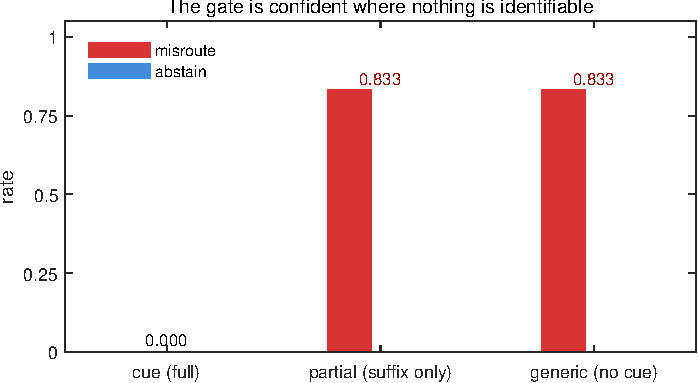
\includegraphics[width=0.70\textwidth]{figures/fig1_cue_ladder.pdf}
\caption{A gate with $1.000$ routing accuracy on identifiable queries is
$\mathbf{0.833}$ confident and $\mathbf{0.000}$ abstinent when nothing in the
query is identifiable. The horizontal axis varies only the cue.}
\label{fig:cue}
\end{figure}

Abstention does not emerge on its own here, but it is cheap to install. The
gate's \texttt{none} class had been trained only on capability-benchmark
prompts and abstained on $0.000$ of cue-free queries. Adding a \emph{single}
cue-free phrasing that shares no surface form with either test condition raises
abstention to $1.000$ and drives misrouting to $0.000$, while the cue-present
condition is untouched at $1.000$ and verifiable capability stays at $0.771$
against a base of $0.750$.

A second observation from the same system set the tone for everything after.
The classification margin separates cue-present from cue-free queries with AUC
$=1.0000$, and a wide feasible threshold interval exists,
$\tau\in[0.114,0.534]$. Our first calibration, taken from the quantile of the
\emph{canonical} training phrasings, placed $\tau$ at $0.9985$, $1.9\times$
above the usable upper bound, and refused $88.9\%$ of cue-present queries. The
metric was right; its calibration was wrong.

\subsection{Contributions}

\begin{enumerate}[leftmargin=1.4em,itemsep=2pt]
\item \textbf{A criterion for building abstention data} (\S\ref{sec:iso}).
      Counter-example completeness is stated relative to the surface features
      that training and evaluation \emph{share}, together with a test that uses
      only the training set and no ground truth.
\item \textbf{A method} (\S\ref{sec:method}). SIA is a four-step recipe that
      teaches answers and abstentions with ordinary supervised fine-tuning:
      $94$\,s per arm, no reward model, no RL loop.
\item \textbf{A controlled construction that satisfies the criterion, and what
      happens when it does not} (\S\ref{sec:exp}). With the criterion
      satisfied, SIA drives fabrication on unseen entities and unseen phrasings
      to $0.000$ with abstention $1.000$ at no measurable cost to capability.
      The three conditions of \S\ref{sec:conditions} are the criterion's three
      axes, and breaking any one of them collapses the effect to exactly
      $0.000$.
\item \textbf{A metric result that falls out of the construction}
      (\S\ref{sec:pooled}). When one slice carries no gold answers, aggregate
      accuracy ranks the safest model last and a model that fabricates
      everywhere first.
\end{enumerate}

\section{Related work}
\label{sec:related}

\paragraph{Abstention and selective prediction.}
TruthRL \cite{truthrl} optimises truthfulness with RL, pairing GRPO with a
ternary reward over correct, hallucinated, and abstained responses. R-Tuning
\cite{rtuning} labels training questions by whether the model answers them
correctly and injects \emph{I am not sure} responses. Lin et al.\ \cite{uncert}
teach models to express uncertainty in words and report that this transfers
unevenly across distributions. Seal \cite{seal} introduces an explicit
rejection token for hallucination caused by knowledge misalignment. SEAT
\cite{seat} attacks the dual problem of preserving already aligned abstention
while injecting knowledge. An earlier line is selective prediction and the
question of whether models know what they know
\cite{selective,knowwhat,calib}. SIA shares the skeleton of these methods,
self-labelled abstention examples followed by ordinary SFT. The difference is
one requirement: we make the surface isomorphism of the two slices explicit,
turn it into a criterion, and test it.

\paragraph{Shortcuts, artifacts, and invariance.}
A parallel literature established that models fit dataset-specific regularities
which do not transfer: shortcut learning \cite{geirhos}, annotation artifacts
and surface heuristics in natural language inference
\cite{artifacts,niven,mccoy}, and remedies from invariant risk minimisation and
worst-case group optimisation \cite{irm,groupdro}. This is the closest relative
of our criterion and we do not claim the underlying principle as new. What the
truth-free setting changes is the operational form of the test: with no ground
truth on the slice of interest there is no held-out shift to measure and no
environment label to group by, so the check has to be made on the training
construction itself.

\paragraph{Ablation discipline.}
The three conditions of \S\ref{sec:conditions} were read off practice and are
stated as separately breakable, which is what makes them testable. The positive
control that isolates the mechanism---abstention-only training on a single
template family---is the same device used to detect annotation artifacts in
natural language inference \cite{artifacts,niven}.

\section{Counter-example completeness}
\label{sec:iso}

\subsection{Setting}

Let $x=(e,a)$ be a query (entity $e$, attribute $a$), and partition queries
into $\mathcal{K}$ (the model has information) and $\mathcal{U}$ (it does not).
The goal is a policy that abstains on $\mathcal{U}$ and answers on
$\mathcal{K}$. The correct answer on $\mathcal{U}$ typically does not exist, so
abstention is treated as a class to be learned, not as a correctness target.

\subsection{Surface features and surface-conflicting pairs}

Write $\sigma(x)$ for the \emph{surface features} of a prompt: entity string
and suffix, attribute name, template family, question length, presence of
digits, and the distribution over expected answer shapes. Everything in
$\sigma(x)$ is visible at generation time. Any function of $\sigma(x)$ is a
\emph{surface rule}.

\begin{quote}
\textbf{Definition (surface-conflicting pair).} A pair of training examples
$(x_i,y_i)$ and $(x_j,y_j)$ is \emph{surface-conflicting} if $\sigma(x_i)$ and
$\sigma(x_j)$ are statistically indistinguishable while $y_i\neq y_j$.
\end{quote}

\subsection{The criterion, relative to the evaluation}

The criterion is only meaningful once we say which surface rules could possibly
be used at test time.

\begin{quote}
\textbf{Criterion (counter-example completeness).} Let $\mathcal A\subseteq
\sigma$ be the algebra generated by those surface features whose values are
\emph{shared} between training and evaluation. A training set $D$ is
\emph{counter-example complete relative to the evaluation} if every
$\mathcal A$-measurable rule that holds on $D$ is refuted by at least one
surface-conflicting pair; equivalently, no $\mathcal A$-measurable classifier
significantly better than chance can fit the labels of $D$.
\end{quote}

The restriction to $\mathcal A$ is not cosmetic, and an earlier draft of this
work did not have it. Without it the criterion is too strong: it condemns
constructions that work. The construction of \S\ref{sec:exp} has series names
that are perfectly label-pure, so a rule keyed on the series name fits the
training set at $1.000$; the unrestricted criterion would reject it, yet the
method trained on it abstains correctly on a held-out series. The reason is
that evaluation there is carried out \emph{on a new series}, so the series axis
cannot be used at test time and a rule keyed on it is inert. What matters is
not whether a leaking axis exists, but \textbf{whether the leaking axis is the
evaluation axis}. Section~\ref{sec:limits} records the cost of this choice.

\paragraph{Why this is enough.}
If some $\mathcal A$-measurable rule agrees with every label in the training
set, empirical risk minimisation can fit that set at zero loss using surface
features alone; low training loss then implies nothing about generalisation to
unseen surface patterns. Conversely, if $D$ is counter-example complete, any
hypothesis with low loss on $D$ must depend on information outside
$\mathcal A$. The first half is purely algebraic. The second rests on an
assumption we state rather than prove, namely that the only non-surface
variable correlated with the label is the model's own evidence state. Its role
is to yield a falsifiable prediction: if one surface rule remains unrefuted,
the method's premise is broken. The three interventions of
Table~\ref{tab:conditions} are exactly such tests, and all three collapse to
$0.000$.

\subsection{The operational test}

Feed the features in $\mathcal A$ to a discriminator and cross-validate it on
the training set, using the split the model is evaluated on; write \surfcv{}
for its accuracy. At the majority-class baseline no usable surface rule exists
and the premise holds; well above baseline a rule survived and the premise is
broken. The quantity needs no held-out labels and no forward pass through the
model: it is a property of the construction. Appendix~\ref{app:protocol} gives
the full protocol.

\section{Method: SIA}
\label{sec:method}

\subsection{The M-M-C-M recipe}

\begin{table}[t]\centering\small
\caption{The four steps of SIA.}
\label{tab:mmcm}
\begin{adjustbox}{max width=\linewidth}
\begin{tabular}{@{}clp{0.68\textwidth}@{}}
\toprule
Step & Name & Operation \\
\midrule
\textbf{M} & \textbf{Measure} &
Define ``has information'' from the model's own sampling self-consistency,
with no ground truth. Sample $k=3$ at $T=0.9$ with a neutral phrasing $P_0$:
gold exists and all three samples match it $\Rightarrow\mathcal{K}$; no gold and
the three samples differ $\Rightarrow\mathcal{U}$; otherwise discard. \\
\textbf{M} & \textbf{Match} &
Build the evidence-free slice to share surface structure with the answer slice:
same entity, same fields, same suffixes, same phrasing shapes. \\
\textbf{C} & \textbf{Cross} &
Answer and abstention examples share one set of templates. This is the heaviest
step, and \S\ref{sec:cross} explains why. \\
\textbf{M} & \textbf{Mix} &
Both kinds of example in one batch, one loss, plain SFT. No RL loop, no reward
model. \\
\bottomrule
\end{tabular}
\end{adjustbox}
\end{table}

\subsection{Where ``Cross'' came from}
\label{sec:cross}

Of the four steps the third carries the most weight, and it was not designed but
forced on us. The first round ran on a synthetic slice in which the supported
set is $4$ series $\times$ $3$ entities $\times$ $5$ fields $=60$ facts, answers
are taught on templates F1 and F2 and evaluated on F4, which is never used for
training, and the value ranges are disjoint so that any numeric answer is
fabricated.

Three readings followed. Abstention does not emerge on its own: an arm trained
on answers alone fabricates at $1.000$. Prompting does not work; a system
prompt telling the model to say it does not know moved fabrication from $0.933$
to $1.000$. And abstention was perfect on the trained phrasings ($1.000$) but
transferred not at all to the unseen one ($0.000$), and adding a second
phrasing family of $30$ examples did not help.

The diagnosis is that on the same examples, and only because answer examples
exist under other templates, abstention degenerates into a template lookup. The
decisive evidence is a positive control: an arm trained on abstention examples
alone, $15$ of them, all from a single phrasing family, abstains on $1.000$ of
unseen phrasings while refusing $0.750$ of real capability questions.
Abstention transfer is therefore not the difficulty; what fails is the
\emph{mixed} training, because mixing supplies a surface rule the model can use
instead.

Moving the abstention examples onto the same template family as the answers
removes that rule. With the same example count and the same initialisation the
difference is $\Delta=+1.000$ on unseen phrasings, with fabrication falling
from $1.000$ to $0.000$. Entity transfer still failed, however: what was
learned was a list of the training entities. Widening the unknown entities from
one to three fixed that, moving abstention on a fourth, never-seen entity from
$0.000$ to $1.000$ and fabrication from $1.000$ to $0.000$.

\subsection{The three conditions}
\label{sec:conditions}

\begin{table}[t]\centering\small
\caption{The three necessary conditions are three axes of one criterion.
Penalties are measured on the synthetic construction.}
\label{tab:conditions}
\begin{adjustbox}{max width=\linewidth}
\begin{tabular}{@{}p{0.26\textwidth}p{0.12\textwidth}p{0.52\textwidth}@{}}
\toprule
Condition read off practice & Axis & Measured penalty when broken \\
\midrule
Slices share surface structure (fields, suffixes, template shape) &
\textbf{structural} &
Control arm's acquisition drops from $0.667$ to $0.400$. \\
Abstention examples share templates with answer examples & \textbf{lexical} &
Uncrossed: abstention on unseen phrasings \bad{$0.000$}; crossed:
\good{$1.000$}. \\
At least three unknown entities & \textbf{entity} &
One entity: abstention on unseen entities \bad{$0.000$}; three:
\good{$1.000$}. \\
\bottomrule
\end{tabular}
\end{adjustbox}
\end{table}

\begin{figure}[t]\centering
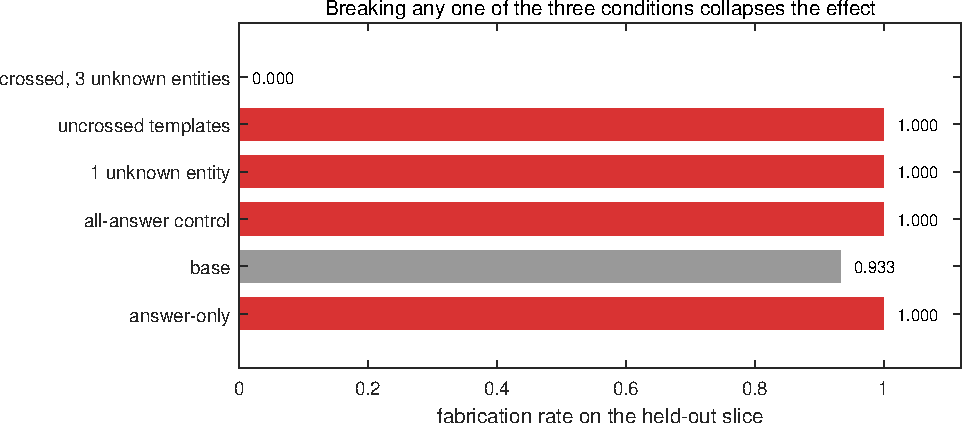
\includegraphics[width=0.84\textwidth]{figures/fig2_conditions.pdf}
\caption{Fabrication on the held-out slice. Only the configuration that
satisfies all three conditions (top, green) reaches $0.000$; breaking any one
of them leaves the model fabricating at $1.000$, as do the answer-only and
all-answer compute controls.}
\label{fig:conditions}
\end{figure}

\subsection{Implementation discipline}

The random initialization of an adapter depends on how many adapters have been
created before it. Holding configuration and seed fixed we measured a
run-to-run variance of roughly $0.5$: a control arm moved from $1.000$ to
$0.480$. The fix is to seed explicitly before creating an adapter. In all
experiments below a single \texttt{zero} adapter is created under a fixed seed,
its matrices are snapshotted, and every arm \texttt{copy\_}s that snapshot back
with a bit-level equality assertion; $\text{init\_gap}=0.0$ throughout.

\section{A controlled construction}
\label{sec:exp}

\subsection{Design}

The training set is the crossed configuration of \S\ref{sec:cross}: supported
series with templates F1/F2 as answers ($120$ items) plus three unknown series
with the same templates as abstentions ($90$ items), $210$ in total. The
evaluation set is a fourth series that appears nowhere in training, queried
with the unseen template F4, together with the supported series under F4:
$75$ items. Crucially, the five field names are \emph{shared} across supported
and unsupported series and the templates are crossed, so the shared algebra
$\mathcal A$ contains no rule that separates the classes.

The base model is Qwen3.5-9B \cite{qwen35}, fine-tuned with LoRA \cite{peft} at
rank $16$ over six layers ($7.012$\,M trainable parameters), $600$ steps at
learning rate $1\times10^{-4}$, batch size $2$, matched initialization. One
training run takes $94$\,s on a single GB10.

\subsection{The construction passes the test}

\begin{table}[t]\centering\small
\caption{\surfcv{} on the construction. Evaluation is carried out on a series
that never appears in training, so the series axis is not in $\mathcal A$.}
\label{tab:surfcv}
\begin{adjustbox}{max width=\linewidth}
\begin{tabular}{@{}lcccc@{}}
\toprule
Features in $\mathcal A$ & $n(\text{answer}/\text{abstain})$ & baseline &
accuracy & gap \\
\midrule
S1 field name & 120/90 & 0.571 & 0.567 $\pm$ 0.030 & \good{$-0.004$} \\
S2 field $+$ template $+$ suffix & 120/90 & 0.571 & 0.571 $\pm$ 0.000 &
\good{$-0.000$} \\
S3 $+$ series name (not in $\mathcal A$) & 120/90 & 0.571 &
1.000 $\pm$ 0.000 & $+0.429$ \\
\bottomrule
\end{tabular}
\end{adjustbox}
\end{table}

A classifier over the shared algebra lands exactly on the majority baseline:
$0.571\pm0.000$ against a baseline of $0.571$, a gap of $-0.000$. The series
axis does leak perfectly, scoring $1.000$, but that axis is not in
$\mathcal A$ because evaluation holds out a series that never appears in
training. There is a further structural point worth recording:
leave-one-series-out is \emph{undefined} on this construction, since every
series is label-pure, with all four supported series labelled answer and all
three unknown series labelled abstention. That is the structural reason the
third condition of Table~\ref{tab:conditions} is needed. It is what gives the
unknown class more than one mutually unrelated value along the entity axis, so
that ``this particular name maps to abstention'' stops being the simplest
explanation consistent with the training set.

\begin{figure}[t]\centering
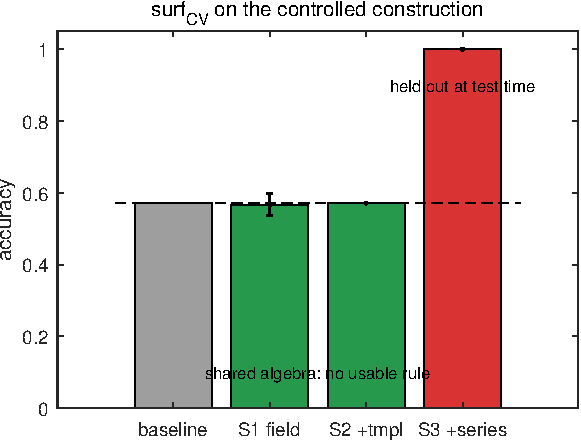
\includegraphics[width=0.62\textwidth]{figures/fig3_surfcv_controlled.pdf}
\caption{\surfcv{} on the controlled construction. The two tiers that use only
shared features sit on the baseline, so no usable surface rule exists; the
series tier is perfect but that axis is held out at test time.}
\label{fig:surfcv}
\end{figure}

\subsection{Main result}

\begin{table}[t]\centering\small
\caption{Controlled construction. \texttt{ans@kn} is accuracy on supported
items; \texttt{abst@new} and \texttt{abst@ent} are abstention rates on unseen
phrasings and on a never-seen entity; \texttt{fabr} is the fabrication rate;
\texttt{pooled} is the aggregate accuracy of \S\ref{sec:pooled}.}
\label{tab:main}
\begin{adjustbox}{max width=\linewidth}
\begin{tabular}{@{}lccccccc@{}}
\toprule
Arm & ans@kn & abst@new & abst@ent & fabr@new & fabr@ent & ans@real & pooled \\
\midrule
\texttt{base} & 0.000 & 0.000 & 0.000 & 0.933 & --- & 0.771 & 0.000 \\
\texttt{sft\_answer\_only} & 0.517 & 0.000 & 0.000 & 1.000 & --- & 0.771 & 0.295 \\
\texttt{sft\_abstain\_only} & 0.000 & 1.000 & 1.000 & 0.000 & --- & 0.146 & 0.000 \\
\midrule
uncrossed templates & 0.450 & 1.000 & 0.000 & 1.000 & --- & 0.771 & 0.257 \\
one unknown entity & 0.483 & 1.000 & 0.000 & 0.000 & 1.000 & 0.750 & 0.242 \\
all-answer compute control & 0.667 & 0.000 & 0.000 & 1.000 & 1.000 & 0.792 & 0.333 \\
\midrule
\textbf{crossed, three unknown} & 0.400 & \good{1.000} & \good{1.000} &
\good{0.000} & \good{0.000} & \good{0.771} & 0.200 \\
\bottomrule
\end{tabular}
\end{adjustbox}
\end{table}

With all three conditions satisfied, abstention is $1.000$ on both held-out
axes and fabrication is $0.000$, while the four configurations that break one
condition or replace abstentions with repeated answers all fabricate at
$1.000$ on at least one held-out axis. Out-of-domain capability stays at the
base level of $0.771$, so there is no measurable over-refusal. Two controls
support the attribution. The compute control holds the example count fixed and
replaces abstention examples with repeated answers; it fabricates at $1.000$,
so the gain is not extra training. The abstention-only arm is the positive
control discussed in \S\ref{sec:cross}: it transfers abstention across
phrasings with $15$ examples, which shows the difficulty lies in the mixed
construction rather than in abstention as a behaviour.

\paragraph{Cost on this construction.}
Abstention examples crowd out acquisition. With three unknown series, $43\%$ of
the training examples are abstentions and $\mathrm{ans}@\text{known}$ falls to
$0.400$; the all-answer control with the same example count reaches $0.667$.
On the real capability questions abstention is $0.000$ and accuracy is $0.771$,
at the base level.

\subsection{Why the metric has to be stratified}
\label{sec:pooled}

The aggregate accuracy column of Table~\ref{tab:main} is not merely
insensitive; it actively penalises safety, and the reason is an identity rather
than a statistical accident. On the unsupported slice there is no gold answer,
so a confident error and a safe abstention are scored identically as zero. The
safest arm in the table, with fabrication $0.000$ on every evidence-free slice
and capability equal to base, has the \emph{lowest} pooled accuracy at $0.200$,
while the control that fabricates on every evidence-free slice has the
\emph{highest} at $0.333$. Any acceptance criterion that aggregates over the
two slices is therefore anti-correlated with the property we are trying to
install, and the abstention and fabrication rates must be reported separately.
This matters beyond bookkeeping: an aggregate-driven development loop will
select against abstention, which is one plausible route by which a model that
passes every benchmark still fabricates on the tail.

\section{Limitations and scope}
\label{sec:limits}

\begin{itemize}[leftmargin=1.4em,itemsep=2pt]
\item \textbf{The evidence is from a controlled construction.} The series,
      fields, and value ranges are synthetic. Establishing the same effect on
      naturally occurring long-tail knowledge is a separate experiment.
\item \textbf{A construction built from real entities fails this criterion.}
      We built one: $160$ real (entity, attribute) pairs with a knowledge
      boundary measured by the model's own sampling self-consistency. It does
      not pass, because its attribute names carry the label---the obscure
      attributes were written with years and precision words and the known ones
      were not, so a discriminator seeing only the attribute name separates the
      two classes at $0.817$ against a $0.510$ baseline. The construction, its
      item-level cost, and the repair are reported in a companion paper; we
      mention it here because a reader should know that the criterion is not
      automatically satisfied by data that looks reasonable.
\item \textbf{The criterion's restriction to shared axes buys self-consistency
      at the price of predictive evidence.} The restriction is motivated by a
      real property---a rule keyed on an axis the evaluation holds out is
      inert---but in this paper the construction was chosen knowing which axis
      is held out. We have not tested the criterion on a case where the choice
      of $\mathcal A$ is not already known, so it is at present a coherent
      definition rather than a validated predictor.
\item \textbf{Single seed per arm.} The separation the paper rests on is
      qualitative---$0.000$ versus $1.000$---and far outside any run-to-run
      variation we observed, but the exact value of the passing arm was
      measured once. The known variance source (adapter creation order) was
      identified and fixed by matched initialisation (\S\ref{sec:method}), and
      multi-seed confirmation of the full grid is not reported here.
\item \textbf{One model, one scale.} $9$B with LoRA $r{=}16$ over six layers,
      on a single GPU. No second model family, no full fine-tuning.
\item \textbf{The boundary construct is model-specific.} It is defined by the
      base model's own sampling self-consistency, so it must be re-measured if
      the base model changes, and there is no guarantee that the resulting
      training set transfers to a different model.
\item \textbf{No inference-time comparison.} We do not compare against a linear
      probe on hidden states, which would test whether abstention is decodable
      without any fine-tuning and therefore how much of the effect is SFT.
\end{itemize}

\section{Conclusion}
\label{sec:conclusion}

We gave a criterion for constructing abstention data without ground truth,
stated relative to the surface features that training and evaluation share, and
a test for it that uses only the training set. The criterion is not a slogan:
the three conditions we originally read off practice are its three axes, and
breaking any one of them collapses the effect to exactly $0.000$.

On a controlled construction that passes the test, SIA drives the fabrication
rate on unseen entities and unseen phrasings from $0.933$ to $0.000$ and
abstention from $0.000$ to $1.000$, using ordinary supervised fine-tuning at
$94$\,s per arm, with no reward model, no RL loop, and verifiable capability
unchanged at the base level. Compute-matched and abstention-only controls
isolate the mechanism: the difficulty is not learning to abstain, it is
preventing the mixed construction from supplying a surface rule instead.

The construction also makes a measurement point that we did not expect to be as
sharp as it is. When one of the two slices carries no gold answers, aggregate
accuracy scores a confident error and a safe abstention identically, so it
ranks the safest model in the table last and a model that fabricates everywhere
first. On this problem, stratified reporting is not a presentational choice.

\appendix

\section{The \surfcv{} protocol}
\label{app:protocol}

Write $\sigma(x)$ down explicitly: entity string and suffix, attribute name,
template family, question length, presence of digits, and the distribution over
expected answer shapes. Restrict it to the features whose values are shared
between the training and evaluation splits, giving $\mathcal A$. Fit a logistic
regression with an L2 penalty over character unigrams and bigrams of the
attribute name, plus explicit style flags (length, presence of a four-digit
year, presence of an exactness word, of a quantity word, or of the ordinal
pattern), plus the entity string in the third tier. Cross-validate $5$-fold
stratified on the training side with $R=10$ repetitions, selecting the ridge
penalty by an inner three-fold. Report accuracy against the majority-class
baseline, which is the quantity that matters, together with AUC. Run it once
per tier, and once with the entities held out entirely: a rule that survives
leave-one-entity-out is not memorisation.

The check is a property of the construction, not of the model, so it runs
without inference. Implementation: \texttt{exp/surf\_cv.m} (MATLAB R2023a,
Statistics and Machine Learning Toolbox); input export in
\texttt{exp/mk\_surf\_inputs\_syn.py}; raw output in
\texttt{exp/out/surf\_cv\_result.json}.

\section{Metrics}
\label{app:metrics}

\begin{itemize}[leftmargin=1.4em,itemsep=1pt]
\item $\mathrm{ans}@\text{known}$: exact-match accuracy on supported items
      queried with unseen phrasings.
\item $\mathrm{abstain}@\text{new}$, $\mathrm{abstain}@\text{ent}$: abstention
      rates on unseen phrasings and on a never-seen entity.
\item $\mathrm{fabricate}@\text{new}$, $\mathrm{fabricate}@\text{ent}$:
      fabrication rates on those two held-out axes. In this construction the
      value ranges of the two classes are disjoint, so any numeric answer is
      fabricated by construction.
\item $\mathrm{ans}@\text{realworld}$: out-of-domain verifiable capability
      (math $24$ plus format $24$). It measures the external cost of
      over-refusal and is insensitive to in-domain over-refusal.
\item \texttt{pooled}: aggregate accuracy over supported and unsupported items
      together. It is reported only to make the point of \S\ref{sec:pooled}.
\end{itemize}

\section{Supplementary readings}
\label{app:readings}

\subsection{Gate readings}
\label{app:gate}

Eight isomorphic synthetic domains, $N$ from $2$ to $8$, routing accuracy
$1.000$ throughout (a factor of $3\times$ to $9\times$ over chance) with zero
misrouting of general text. The cue ladder ($N=6$, \texttt{argmax}, no
abstention mechanism):

\begin{center}\small
\begin{adjustbox}{max width=\linewidth}
\begin{tabular}{@{}lcccc@{}}
\toprule
Condition & route\_acc & abstain & misroute & median margin \\
\midrule
\texttt{cue} (positive control) & 1.000 & 0.000 & 0.000 & 0.8030 \\
\texttt{partial} & 0.167 & 0.000 & 0.833 & 0.0223 \\
\texttt{generic} & 0.167 & 0.000 & 0.833 & 0.0203 \\
\texttt{coref}, full context & 1.000 & 0.000 & 0.000 & 0.6686 \\
\texttt{coref}, current turn only & 0.278 & 0.722 & 0.000 & --- \\
\bottomrule
\end{tabular}
\end{adjustbox}
\end{center}

The two margin groups have disjoint intervals, giving AUC $=1.0000$. The
feasible threshold interval is $\tau\in[0.1142,0.5335]$; calibrating on
canonical phrasings places $\tau$ at $0.9985$ and refuses $88.9\%$ of
cue-present queries, against $0.000$ when $\tau$ comes from a same-family
validation set. The abstention class, trained on the gate's \texttt{none} class:

\begin{center}\small
\begin{adjustbox}{max width=\linewidth}
\begin{tabular}{@{}lccccc@{}}
\toprule
Training data for \texttt{none} & cue correct & generic abstain &
generic misroute & partial abstain & partial misroute \\
\midrule
Capability prompts only & 1.000 & 0.000 & 0.833 & 0.000 & 0.833 \\
$+T_c$ (one phrasing, never tested) & 1.000 & 1.000 & 0.000 & 1.000 & 0.000 \\
$+T_a+T_b+T_c$ & 1.000 & 1.000 & 0.000 & 1.000 & 0.000 \\
\bottomrule
\end{tabular}
\end{adjustbox}
\end{center}

Capability is unharmed: $0.771$ under per-domain routing against a base of
$0.750$, with LM CE $1.4962$.

\subsection{Construction readings}
\label{app:synth}

Round one, uncrossed templates (Qwen3.5-9B, LoRA $r{=}16$).
\texttt{base\_prompt} appends a system instruction telling the model to say it
does not know; \texttt{sft\_abstain\_1fam} and \texttt{sft\_abstain\_3fam} add
$15$ and $30$ abstention examples; \texttt{sft\_abstain\_only} trains on
abstention examples alone and is the positive control, reaching $0.146$
accuracy on real capability questions while abstaining on $0.750$ of them.

\begin{center}\small
\begin{adjustbox}{max width=\linewidth}
\begin{tabular}{@{}lccccc@{}}
\toprule
Arm & ans@F4 & abst@F3 & abst@F4 & fabr@F4 & ans@real \\
\midrule
\texttt{base} & 0.000 & 0.000 & 0.000 & 0.933 & 0.771 \\
\texttt{base\_prompt} & 0.000 & 0.000 & 0.000 & 1.000 & 0.771 \\
\texttt{sft\_answer\_only} & 0.517 & 0.000 & 0.000 & 1.000 & 0.771 \\
\texttt{sft\_abstain\_1fam} & 0.433 & 1.000 & 0.000 & 1.000 & 0.792 \\
\texttt{sft\_abstain\_3fam} & 0.433 & 1.000 & 0.000 & 1.000 & 0.771 \\
\texttt{sft\_abstain\_only} & 0.000 & 1.000 & 1.000 & 0.000 & 0.146 \\
\bottomrule
\end{tabular}
\end{adjustbox}
\end{center}

Round two, crossed templates, $150$ examples per arm, matched initialisation:

\begin{center}\small
\begin{adjustbox}{max width=\linewidth}
\begin{tabular}{@{}lccccc@{}}
\toprule
Arm & ans@kn & abst@F3 & abst@F4 & fabr@F4 & ans@real \\
\midrule
\texttt{sft\_blocked\_2fam} (separable) & 0.450 & 1.000 & 0.000 & 1.000 & 0.771 \\
\texttt{sft\_cross\_2fam} (crossed) & 0.467 & 1.000 & 1.000 & 0.000 & 0.750 \\
\texttt{sft\_more\_answer30} (compute control) & 0.700 & 0.000 & 0.000 & 1.000 & 0.750 \\
\bottomrule
\end{tabular}
\end{adjustbox}
\end{center}

Round three, unknown-entity diversity, evaluated on a fourth never-seen entity:

\begin{center}\small
\begin{adjustbox}{max width=\linewidth}
\begin{tabular}{@{}lccccccc@{}}
\toprule
Arm & ans@kn & abst@new & abst@ent & fabr@new & fabr@ent & ans@real & pooled \\
\midrule
\texttt{sft\_cross\_1unk} & 0.483 & 1.000 & 0.000 & 0.000 & 1.000 & 0.750 & 0.242 \\
\texttt{sft\_cross\_3unk} & 0.400 & 1.000 & 1.000 & 0.000 & 0.000 & 0.771 & 0.200 \\
\texttt{sft\_cross\_3unk\_ctrl} & 0.667 & 0.000 & 0.000 & 1.000 & 1.000 & 0.792 & 0.333 \\
\bottomrule
\end{tabular}
\end{adjustbox}
\end{center}

\section{Code and reproduction}
\label{app:repro}

Code and data are at
\url{https://github.com/forrestsong/Surface-Isomorphic-Abstention-exp}.
The commands below produce the readings in Appendix~\ref{app:readings}.

\begin{verbatim}
git clone https://github.com/forrestsong/Surface-Isomorphic-Abstention-exp
cd Surface-Isomorphic-Abstention-exp/exp

# Python 3.11, torch 2.13.0+cu130, single DGX Spark (GB10, 121 GiB unified)
G3_12_PROFILE=main     python g3_12_abstain_method.py   # round one
G3_12_PROFILE=cross    python g3_12_abstain_method.py   # round two
G3_12_PROFILE=multiunk python g3_12_abstain_method.py   # round three

python mk_surf_inputs_syn.py                            # criterion check
matlab -batch "run('surf_cv.m')"
matlab -batch "run('make_figs.m')"
\end{verbatim}

\begin{thebibliography}{99}

\bibitem{truthrl} Z.~Wei \emph{et al.},
  ``TruthRL: Incentivizing Truthful LLMs via Reinforcement Learning,''
  arXiv:2509.25760, 2025.

\bibitem{rtuning} H.~Zhang \emph{et al.},
  ``R-Tuning: Instructing Large Language Models to Say `I Don't Know',''
  in \emph{Proc. NAACL}, 2024.

\bibitem{uncert} S.~Lin, J.~Hilton, and O.~Evans,
  ``Teaching Models to Express Their Uncertainty in Words,''
  \emph{TMLR}, 2022.

\bibitem{seal} L.~Huang \emph{et al.},
  ``Alleviating Hallucinations from Knowledge Misalignment in Large Language
  Models via Selective Abstention Learning,''
  in \emph{Proc. ACL (Long Papers)}, pp.~24564--24579, 2025.

\bibitem{seat} W.~F.~Shen, X.~Qiu, N.~Cancedda, and N.~D.~Lane,
  ``SEAT: Sparse Entity-Aware Tuning for Knowledge Adaptation while Preserving
  Epistemic Abstention,'' arXiv:2506.14387, 2025.

\bibitem{peft} S.~Mangrulkar \emph{et al.},
  ``PEFT: Parameter-Efficient Fine-Tuning of Billion-Scale Models,'' 2022.

\bibitem{qwen35} Qwen Team, ``Qwen3.5 Technical Report,'' 2025.

\bibitem{selective} Y.~Geifman and R.~El-Yaniv,
  ``Selective Classification for Deep Neural Networks,'' in \emph{NeurIPS}, 2017.

\bibitem{knowwhat} Z.~Yin \emph{et al.},
  ``Do Large Language Models Know What They Don't Know?,''
  in \emph{Findings of ACL}, 2023.

\bibitem{calib} S.~Kadavath \emph{et al.},
  ``Language Models (Mostly) Know What They Know,'' arXiv:2207.05221, 2022.

\bibitem{geirhos} R.~Geirhos \emph{et al.},
  ``Shortcut Learning in Deep Neural Networks,''
  \emph{Nature Machine Intelligence}, vol.~2, pp.~665--673, 2020.

\bibitem{artifacts} S.~Gururangan \emph{et al.},
  ``Annotation Artifacts in Natural Language Inference Data,''
  in \emph{Proc. NAACL}, 2018.

\bibitem{niven} T.~Niven and H.-Y.~Kao,
  ``Probing Neural Network Comprehension of Natural Language Arguments,''
  in \emph{Proc. ACL}, 2019.

\bibitem{mccoy} R.~T.~McCoy, E.~Pavlick, and T.~Linzen,
  ``Right for the Wrong Reasons: Diagnosing Syntactic Heuristics in Natural
  Language Inference,'' in \emph{Proc. ACL}, 2019.

\bibitem{irm} M.~Arjovsky, L.~Bottou, I.~Gulrajani, and D.~Lopez-Paz,
  ``Invariant Risk Minimization,'' arXiv:1907.02893, 2019.

\bibitem{groupdro} S.~Sagawa, P.~W.~Koh, T.~B.~Hashimoto, and P.~Liang,
  ``Distributionally Robust Neural Networks for Group Shifts: On the Importance
  of Regularization for Worst-Case Generalization,'' in \emph{ICLR}, 2020.

\end{thebibliography}

\end{document}
